

\documentclass[final,a4paper,oneside,12pt]{article}
\setlength{\parindent}{0in}
 \usepackage{verbatim}
\usepackage{amsfonts}
\usepackage{amsmath}
\usepackage{color}
\usepackage{amssymb}
\usepackage[pdftex]{graphicx}
\begin{comment}
\usepackage[OT2,T1]{fontenc}
\DeclareSymbolFont{cyrletters}{OT2}{wncyr}{m}{n}
\DeclareMathSymbol{\Sha}{\mathalpha}{cyrletters}{"58}
\end{comment}
\usepackage{geometry}
%% Alex's thing
\setlength{\parskip}{0pt}
\setlength{\parsep}{0pt}
\setlength{\headsep}{0pt}
\setlength{\topskip}{0pt}
\setlength{\topmargin}{0pt}
\setlength{\topsep}{0pt}
\setlength{\partopsep}{0pt}
\linespread{1}

\geometry{
  body={7in, 10in},
  left=0.6in,
  top=0.5in
}

\setlength\parindent{0em}

\usepackage[compact]{titlesec}
\titlespacing{\section}{0pt}{*1}{*1}
\titlespacing{\subsection}{1pt}{*0.8}{*0.8}
\titlespacing{\subsubsection}{0pt}{*0}{*0}

\usepackage{amsfonts}
\usepackage{amsmath}
\usepackage{amssymb}
\usepackage[pdftex]{graphicx}
\usepackage{fullpage}
%%%
\begin{document}

\centerline{\Large \bf{Iron Concentration Plotter User Manual}}
\bigskip
\centerline{James McMurray}
\bigskip

\renewcommand{\labelenumi}{{\color{red} {\bf\arabic{enumi}}}}

\section{QSSPC Measurements - GUI Map}

When the program is first loaded the default tab is the ``QSSPC'' tab. Figure \ref{figure1} shows this window labelled when in use.

\begin{figure}[h]
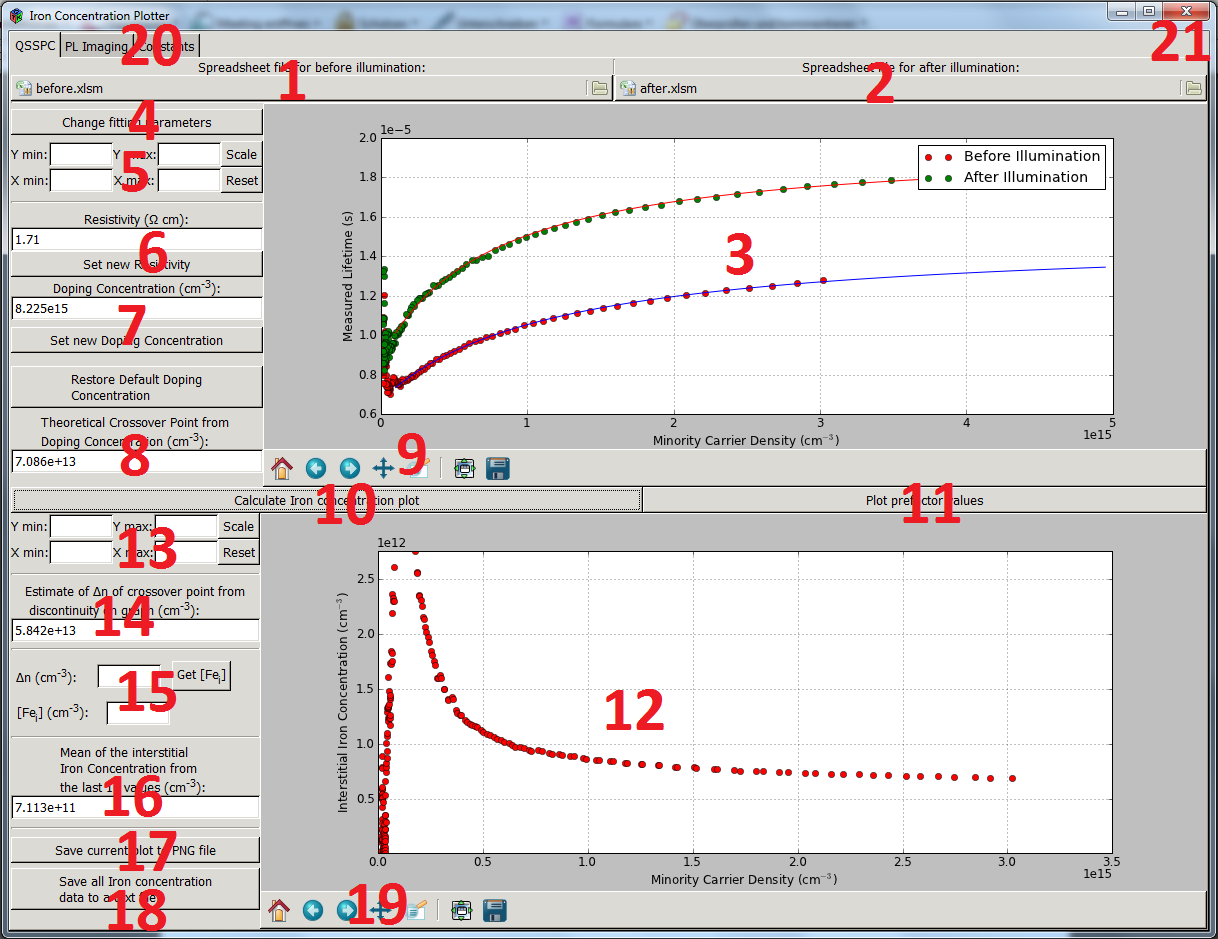
\includegraphics[height=5in]{2mainscreen}
\caption{\label{figure1} The QSSPC tab shown after loading the Excel files and plotting the graph of interstitial Iron Concentration.}
\end{figure}

\begin{enumerate}
\item The button used to load the Excel file for before illumination. The file loaded must be of .XLSM format and the program will check it can be loaded correctly.

\item The button used to load the Excel file for after illumination.

\item The area where the lifetime against injection level graphs (QSSPC measurements) are plotted from the Excel files. Hovering over it will give the X and Y values in the navigation toolbar below.

\item This button opens a window where the initial guess for the fits can be changed and the actual parameters plotted viewed.

\item Text boxes where the view window of the graph can be manually set. The numbers can be edited as they are on the graph i.e. X minimum as 1 and X maximum as 2, rather than 1e15 and 2e15 respectively, this is useful when zooming. However, this can occasionally cause problems (especially with graphs which have negative values), at which point the full specification with the exponent should be used. One box can be edited individually to change one part of the scale independently of the others.

\item  Here the Resistivity is read from the Excel file, and the Doping Concentration is calculated from it. The Resistivity value may be edited and the ``Set new Resistivity'' button used to set it and calculate the new Doping Concentration.

\item Here the calculated Doping Concentration is printed. The Doping Concentration may then be edited here to override the calculated value for calculating the interstitial Iron Concentration graph and the Photo-Luminescence (PL) maps.

\item Here a theoretical value is calculated for the Cross-Over Point (COP) from the Doping Concentration value using the equation given in Birkholz \textit{et al.} JAPL {\bf 97}, 103708 (2005), note that this does not take temperature dependence in to account and so may be inaccurate for this reason.

\item The navigation toolbar for the QSSPC graph. The home button resets the view to default, or to the manually set value using the manual controls marked at {\color{red}{\bf 5}}. The back and forward buttons move between views that the user has set using the pan or zoom tool, like the Back/Forward buttons in a Web Browser, it does not pan itself. The panning tool pans across the graph by holding the leftm mouse button on the graph and dragging the mouse cursor in the opposite direction to the panning. The Zoom tool allows the user to click and draw a rectangle on the graph to zoom to. The Configure Subplots button adjusts the borders of the plot, this may be useful when saving. The save button allows the current plot to be saved.

\item This button calculates and plots the Iron Concentration graph.

\item This button calculates and plots the Prefactor values graph. It also changes controls {\color{red} {\bf 13}}, {\color{red} {\bf 15}}, {\color{red} {\bf 16}} and {\color{red} {\bf 17}} to work for the Prefactor values.

\item This is the area where the Iron Concentration plot is loaded. It behaves the same as the lifetime plot.

\item This is the area where the view can be set manually for the Iron Concentration/Prefactor values plot, it behaves the same as {\color{red} {\bf 5}}.

\item Here the COP is calculated from the graph as the point between the maximum Iron Concentration value and the next value (as the Iron Concentration tends to infinity at the COP).

\item Here a value for the injection level can be entered and the interstitial iron concentration value at this point will be printed.

\item Here the mean value of the last 10 values (i.e. highest injection level, so stable) of either the Iron Concentration or Prefactor values will be printed (depending on which graph is the actively plotted one).

\item This button saves the current plot to a PNG file, it is identical to the button in the navigation toolbars except it only supports PNG files.

\item This button saves the iron concentration plot data to a text file.

\item The Navigation Toolbar for the Iron Concentration graph. This behaves the same way as {\color{red} {\bf 9}}.

\item Here the other tabs can be opened for the PL Imaging and modifying the constants used in all calculations.

\item Here the application can be closed, maximised or minimised.
\end{enumerate}

\section{PL Imaging}
\subsection{GUI Map}

\begin{figure}[h]
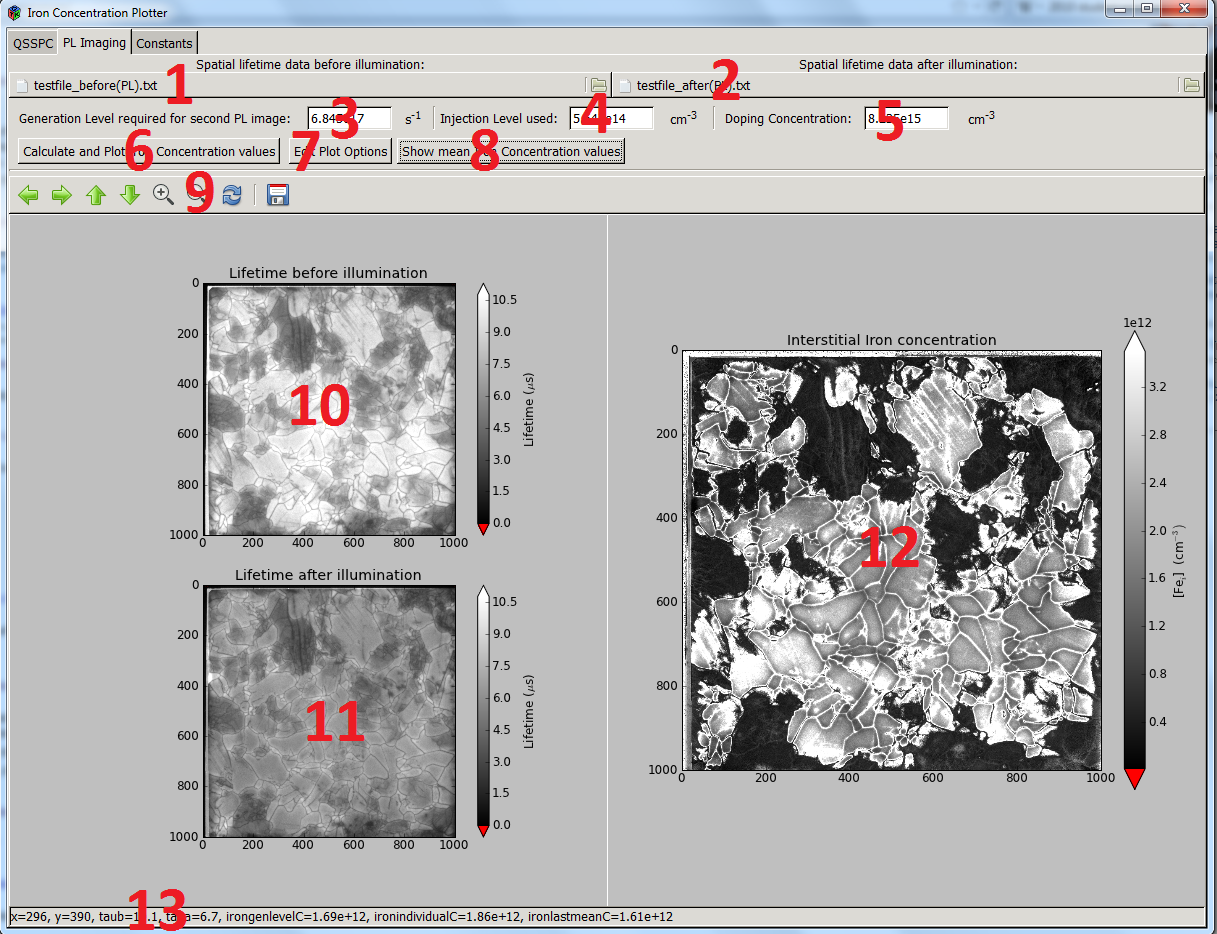
\includegraphics[height=4in]{2plimaging}
\caption{\label{figure2} The PL imaging tab shown after loading the PL data files and plotting the PL maps for lifetime and interstitial iron concentration.}
\end{figure}

\begin{enumerate}
\item Here the PL data file for before illumination is selected. After selection a box will appear asking for the generation level used for this PL image, to determine the generation level required for the second PL image from the Excel files loaded in the QSSPC page.
\item Here the PL data file for after illumination is selected, the selection window lists the required generation level in the window title so it is easily viewable.
\item  Here the desired Generation Level for the after illumation PL data is listed so it can be read whilst selecting the file.
\item Here the injection level used in the calculation of the Iron Concentration PL Map is shown, and may be edited. It is read from the injection level corresponding to the given generation level in the Before Illumination Excel file.
\item Here is the Doping Concentration level, it is read from the Excel file and will be updated if it is changed on the QSSPC page. It can also be edited here for producing the PL maps.
\item This button calculates and plots the iron concentration values, and then asks whether adjustment of the lifetime images is necessary. It may take a long time.
\item This button opens a window where the colorbar colormap can be changed, the limits on the colorbar can be changed as can whether the maps are base-10 logarithmic or linear and the type of calculation used for the interstitial iron concentration map.
\item This button shows a window with the mean interstitial iron concentration values from different calculations.
\item The navigation toolbar, here the arrows are panning buttons, and the panning moves all the maps together to keep them comparable. The zooming function also works this way. The save button opens a dialog asking which plot or data to save.
\item The plot area for the before illumination lifetime map.
\item The plot area for the after illumination lifetime map. Note that both lifetime maps actually belong to the same figure, and so are saved together.
\item The plot area for the interstitial iron concentration map. Note that the iron concentration map is a separate figure from the lifetime figure and so must be saved separately.
\item The status bar, hovering over the plots provides details of the points here. It lists the current x co-ordinate, y co-ordinate, before illumination lifetime (in microseconds), after illumination lifetime, the interstitial iron concentration at the point as calculated using the prefactor calculated from the given generation level, the interstitial iron concentration at the point as calculated using the individual prefactor for that point (by matching the lifetimes to the QSSPC fits to get an injection level), and the interstitial iron concentration at the point by using the mean of the high prefactors calculated from the QSSPC graph.
\end{enumerate}


\section{User Guide}
{\bf To fix graphical glitches try making the window full size after running the program.}\\
The Excel files are loaded using the two buttons at the top of the screen and the QSSPC lifetime data is plotted. The resistivity (or doping concentration directly) can then be changed manually if desired. The fits can also be adjusted to ensure the values used for calculating the individual prefactor values for the PL images are accurate, and the actually used fit parameters can be viewed in the ``Change Fitting Parameters'' window along with the square root of the sum of the squared differences of the fit and actual values (ie. $\sqrt{\sum (y_{fit} - y_{actual})^{2}}$) as an estimate for the error in the fit. Note that this is only calculated {\bf for the given fitting range}, and so a poor overallfit with a small fitting range could have a very low error. The Resistivity and Doping Concentration used can also be varied manually (the former is used to calculate the latter).\\

Note that if the Before Illumination data covers a smaller range than the After Illumination data then the fit will not be plotted all the way, refreshing the plot by loading the Edit Fit window and clicking OK or clicking the calculate Iron Concentration plot Button will fix it. Note that this has no effect on the calculations anyway.\\

When the ``Use fits or interpolation'' box is set to ``Use fits'', the calculation of the interstitial iron concentration and C factor values will use the fits to the QSSPC values, when it is set to ``Use interpolation'' it will use the linear interpolation of the measured values. Use this if the fit is bad and this cannot be rectified by adjusting the initial guesses. If the fit is bad then the PL map of the interstitial Iron concentration using individual C factor values for each pixel should be ignored as the values will be untrustworthy.
\\
The interstitial Iron Concentration against injection level plot can then be calculated and plotted, as can the prefactor values against injection level. The relevant data can be saved to a text file, this includes the QSSPC data, the fitting data and the iron concentration data. The mean of the iron concentration and prefactor values between a given range can be calculated, {\bf this range is then used for the mean calculation for the ``Use mean C value in given range'' PL Map}. After clicking the ``Calculate Iron Concentration plot'' button the program will also attempt to get the crossover-point from the QSSPC fits by solving a quadratic, if the values are negative then it means there is no cross-over point on the fits and should be ignored.
\\
The plot itself can be saved using the Disk icon on the Navigation Toolbar. Note that the arrows on the toolbar do not represent panning, but rather back and forward frame buttons, like on a Web Browser. Panning is achieved with the Panning icon. The Configure Subplots icon lets one set the borders of the plot.\\

The PL Imaging tab is then opened. Then the PL before illumination data file can be selected, and the generation level used can be entered in to the dialog box.

\begin{figure}[h!]
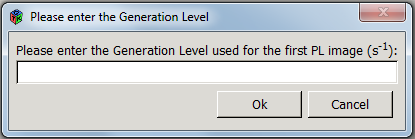
\includegraphics[height=1in]{2genlevel}
\caption{\label{figure2} The window where the user enters the generation level used for the Before Illumination PL image.}
\end{figure}

The PL after file is then chosen with the generation level closest to that given in the filled textbox and dialog title.

\begin{figure}[h!]
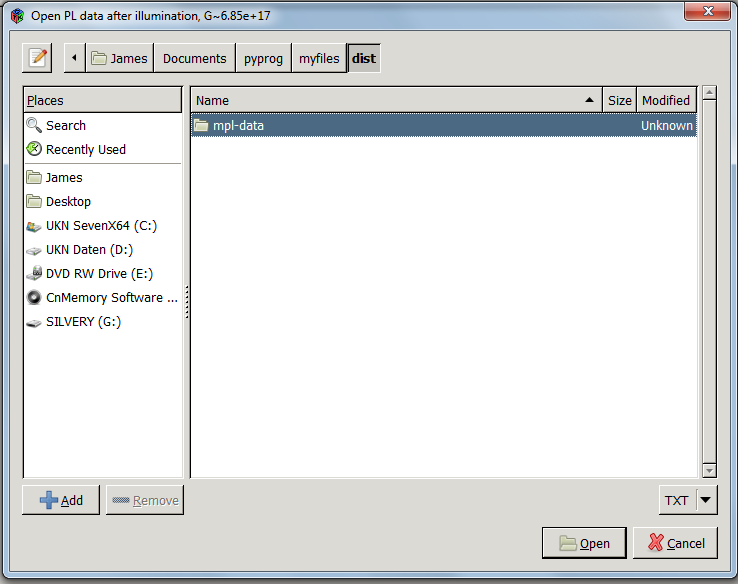
\includegraphics[height=3in]{2loadplafterfile} 
\caption{\label{figure2} The window where the After Illumination PL file is loaded, note the target generation level is given in the window title.}
\end{figure}


 The PL maps may then be calculated and plotted. The default maps plotted have linear scales and the interstitial iron map plotted is using the individual prefactor values for each pixel. Negative lifetime values are set to -6E30 so they appear red on the lifetime maps. The program then asks the user whether they wish to attempt adjusting the after illumination lifetime map to ensure that the pixels are in the right position compared to the before illumination map.\\

\begin{figure}[h!]
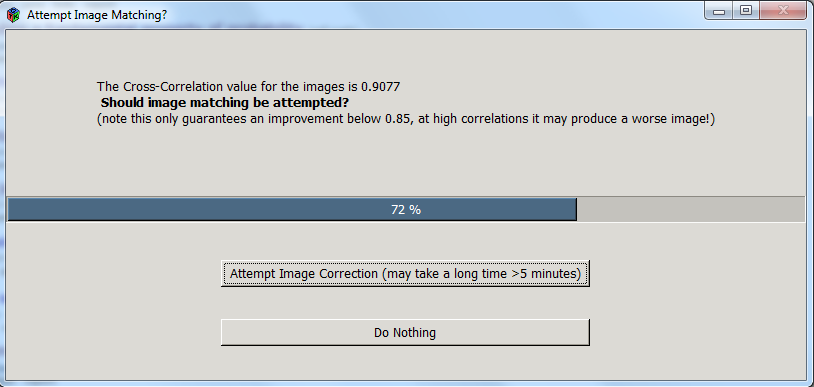
\includegraphics[height=2in]{2attemptcorrection}
\caption{\label{figure2} The window which asks whether image correction should be attempted. Here it has been and the progress bar is shown during the calculation process.}
\end{figure}

If this is done then it will make the calculated adjustments to maximise the correlation, and the user is given the option to save the adjusted data. When it is completed a window will show the results of the transformation on the cross-correlation value and the user has the opportunity to save the adjusted After Illumination lifetime data. The lifetime data can also be saved using the Disk icon on the Navigation Toolbar for the PL maps.

\begin{figure}[h!]
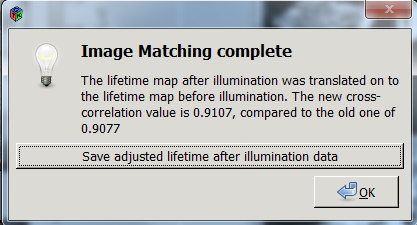
\includegraphics[height=2in]{2imagematchingcomplete}
\caption{\label{figure2} The window shown when image matching is complete. The cross-correlation values are given and the user has an opportunity to save the adjusted lifetime data.}
\end{figure}

%\pagebreak

When calculating the C factor for each pixel, the program takes the lifetime values for the pixel, before and after illumination, and uses the fits to get injection level values from these. If the values differ by more than the warning value (set in the Edit Plot Options window) then they will be flagged as red, as the injection level difference is considered too high for them to be trustworthy. To colour them red, the values are set to -7E30. Values are also set red if the lifetime values were negative or zero (and so would produce infinities), these values are set to -6E30 and so can be distinguished from the others by hovering over them. Note that the PL maps have to be recalculated after changing the warning level.
\\
The Plot Options can then be changed, to set the limits on the plots, make them logarithmic or linear, change the colour map used and change the type of interstitial iron concentration calculation that is plotted. Note that when using logarithmic scales the limits should not be set equal to, or less than, zero as this will produce errors, nor should boxes be left blank as this may also produce errors. The different color maps all have distinct colors for values below the scale limit to highlight anomalous values.

\begin{figure}[h!]
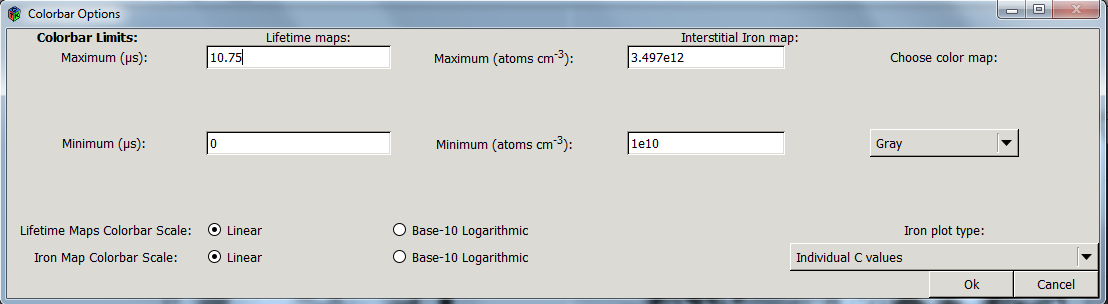
\includegraphics[height=1.8in]{editcolorbar}
\caption{\label{figure2} The plot options window. Note that when the plots are logarithmic the scale values cannot be equal to zero (or negative), and boxes cannot be left unfilled.}
\end{figure}

The mean interstitial Iron Concentration values for the different methods of calculation can be viewed by clicking the ``Show mean Iron Concentration values'' button.

\begin{figure}[h!]
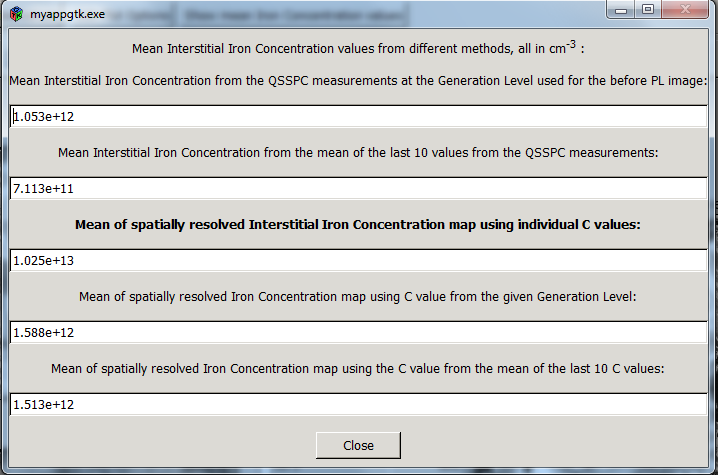
\includegraphics[height=2in]{meanvalues}
\caption{\label{figure2} The window showing the mean interstitial Iron Concentration value from the various calculation methods.}
\end{figure}

The ``Mean Interstitial Iron Concentration from the QSSPC measurements at the Generation Level used for the before PL image'' gives the interstitial iron concentration from the QSSPC measurements at the given generation level (from which the closest injection level is matched). The ``Mean Interstitial Iron Concentration from the mean of the last 10 values from the QSSPC measurements'' takes the mean of the last 10 values on the plotted Iron Concentration graph from the QSSPC measurements as these are stable compared with the lower-injection level values. The ``{\bf Mean of spatially resolved Interstitial Iron Concentration map using individual C values}'' takes the mean of the spatially resolved interstitial Iron Concentration map when the prefactor for the calculation is calculated seperately for each pixel by taking the Before Illumination and After Illumination lifetimes and obtaining an injection level by seeing where these appear on the QSSPC fits, this injection level is then used to calculate the prefactor for that pixel. If the lifetimes are too low to be fitted then the minimum injection level from the QSSPC plot is used. The ``Mean of spatially resolved Iron Concentration map using C value from the given Generation Level'' uses the given generation level to obtain an injection level by finding the closest value in the Before Illumination file, and then uses this to calculate a prefactor value which is applied to all pixels. The ``Mean of spatially resolved Iron Concentration map using the C value from the mean of the last 10 C values'' takes the mean of the last 10 C values on the C value (prefactor) plot from the QSSPC measurements and applies this C factor to all the pixels.


\begin{figure}[h!]
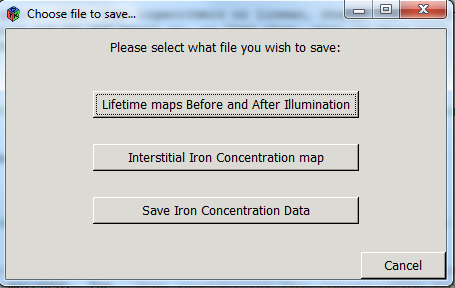
\includegraphics[height=2in]{2whichsave}
\caption{\label{figure2} From this window the user can save the different PL data sets. The first two are images, whilst the last is the actual calculated Interstitial Iron Concentration data set, it will save whatever type of calculation is currently plotted.}
\end{figure}

The user can also click the save button in the Navigation Toolbar of the PL maps to save images of the plots as they are, and also to save the calculated interstitial iron concentration data to a file. The data saved will be whatever calculation method is currently plotted.
\\

Finally, the constants used in the calculation of the prefactor values can be modified on the Constants window as shown. Note that they only take effect at the next calculation, so if already plotted, the graphs will need to be recalculated.

\begin{figure}[h!]
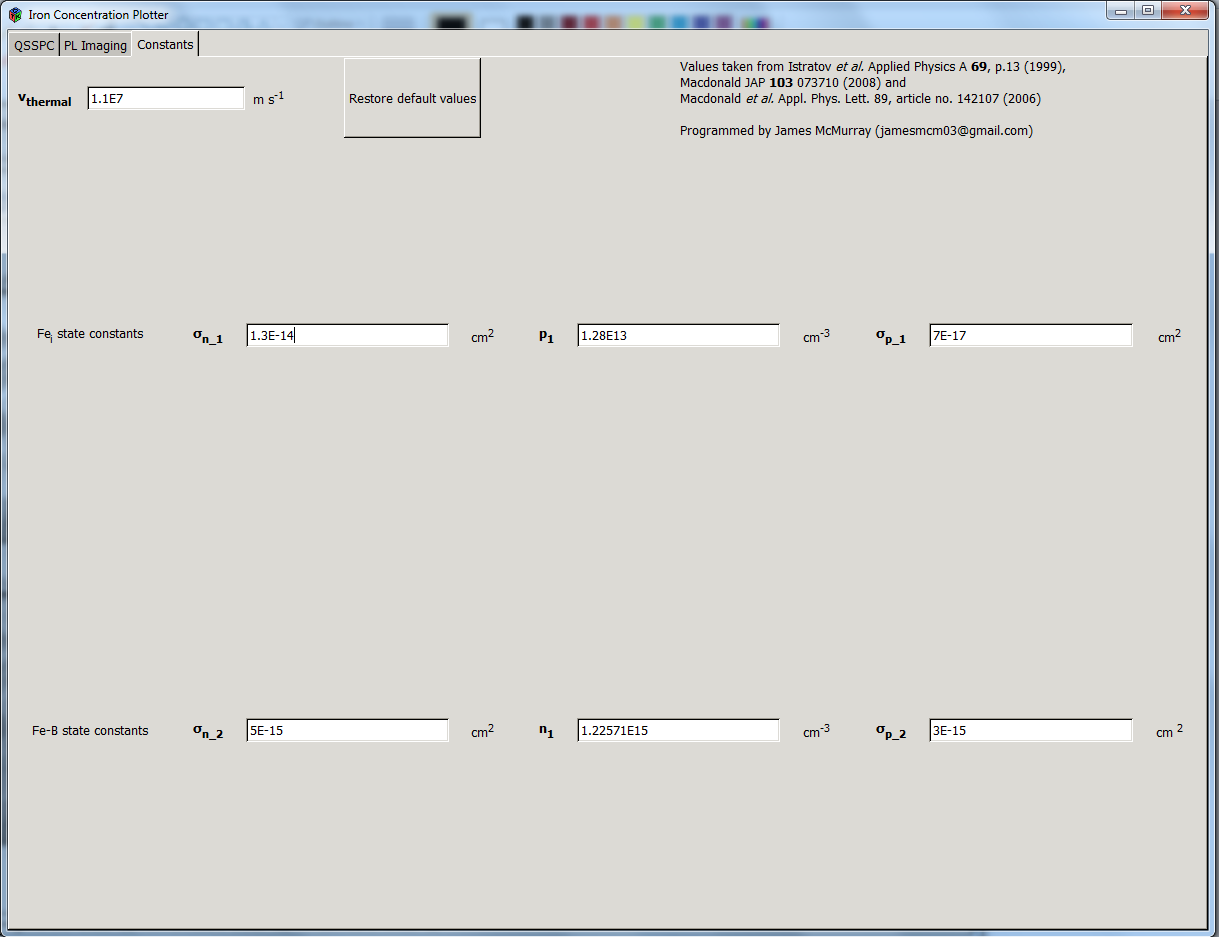
\includegraphics[height=4in]{2constants}
\caption{\label{figure3} The Constants tab, here the constants can be edited.}
\end{figure}


\end{document}







